\documentclass[11pt]{article}
\usepackage[hyperref]{acl}
\usepackage{times}
\usepackage{latexsym}
\usepackage{microtype}
\usepackage{booktabs}
\usepackage{multirow}
\usepackage{graphicx}
\usepackage{amsmath}
\usepackage{amssymb}
\usepackage{listings}
\usepackage{xcolor}
\usepackage{enumitem}
\usepackage{tabularx}
\usepackage{array}
\usepackage{pifont}
\usepackage{tikz}
\usetikzlibrary{arrows.meta,positioning,shapes.geometric,fit,backgrounds,calc}

\lstset{
  basicstyle=\ttfamily\scriptsize,
  breaklines=true,
  frame=single,
  backgroundcolor=\color{gray!8},
  commentstyle=\color{gray},
  keywordstyle=\color{blue},
  aboveskip=4pt,
  belowskip=4pt,
}

\title{UnMask: Mastery-Gated Retrieval for Socratic OT Anatomy Education}

\author{Sanika Vilas Najan \quad Vaishak Girish Kumar \\
  University at Buffalo \\
  CSE 635: NLP and Text Mining --- Spring 2026 \\
  Instructor: Prof.\ Rohini K.\ Srihari \\
  \texttt{\{snajan, vaishakg\}@buffalo.edu}}

\begin{document}
\maketitle

%% ─────────────────────────────────────────────────────────────
\begin{abstract}
We built \textbf{UnMask}, a Socratic AI tutor for OT anatomy NBCOT prep.
Most Socratic AI tutors try to suppress answers at generation time, but
we moved this to the \emph{retrieval layer} using \textbf{Progressive Context Revelation (PCR)}:
a metadata-filtered Qdrant query that withholds answer chunks until
the student demonstrates prerequisite mastery.
We also added \textbf{Corrective RAG (CRAG)} (to our knowledge the first use in
educational tutoring), dual-layer structured output masking, and
\textbf{session mistake memory}, a log of wrong answers that triggers a
proactive revisit at 8 minutes using the student's stored misconception.
We evaluated on 30 QA triples with a four-variant ablation: Hit Rate 0.900,
Leak Rate 0.000, Socratic Purity 4.77/5, 100\% adversarial hold rate.
All variants show 0.000 leak under benign conditions, but only PCR
provides safety by design at a measured 0.23-point purity cost (4.70 vs.\ 4.93).
RAGAS Faithfulness (0.779) shows a metric mismatch: RAGAS penalizes
Socratic questions that make no factual claims, which is expected here.
\end{abstract}

%% ─────────────────────────────────────────────────────────────
\section{Introduction}

Occupational Therapy students need to master Gross Anatomy and Neuroscience to
pass the NBCOT exam, but standard AI systems work against this by giving direct answers
and bypassing the clinical reasoning the exam actually tests.
The project spec defines ``Socratic'' tutoring as a \emph{Tutor-not-Teller}
approach: the system should ask guiding questions that lead the student to the answer,
never stating it outright.

The core problem is that prompt-based suppression only works at generation time.
Dinucu-Jianu et al.\ \cite{tutorrl2025} showed larger models have \emph{higher}
leak rates because their parametric knowledge overrides system prompts.
The only reliable fix is to keep the LLM from ever receiving the answer.

\paragraph{Our main claim.}
By filtering retrieval using student mastery, answer leakage becomes
impossible before mastery thresholds are met. This is enforced by a 10-line
Qdrant metadata filter that no adversarial prompt can get around.

%% ─────────────────────────────────────────────────────────────
\section{Related Work}

Table~\ref{tab:related} summarises the key distinctions.
Dinucu-Jianu et al.\ \cite{tutorrl2025} showed that larger LLMs have
\emph{higher} leak rates because parametric knowledge overrides system prompts, which is what motivated our retrieval-layer approach.
Corrective RAG \cite{crag2024} adds a self-assessment step after retrieval
(+19\% PopQA, +36.6\% PubHealth); no prior work applies CRAG in educational tutoring.
Closest to our retrieval approach is TutorLLM \cite{tutorllm2024}, which combines knowledge tracing with RAG for personalized learning, but does not specify a mastery-gated metadata filtering mechanism. Dinucu-Jianu et al.\ \cite{tutorrl2025} show that RL reward shaping for pedagogical alignment outperforms prompt-based suppression on GPT-4o, consistent with our finding that prompt-level safety fails under adversarial attack.

\begin{table}[h]
\centering
\small
\setlength{\tabcolsep}{4pt}
\begin{tabular}{@{}lccc@{}}
\toprule
\textbf{System} & \textbf{RAG} & \textbf{Mastery gate} & \textbf{Layer} \\
\midrule
Khanmigo         & \checkmark & $\times$ & prompt \\
SocraticLM \cite{socraticlm2024} & $\times$ & $\times$ & fine-tune \\
KELE \cite{kele2025}      & \checkmark & $\times$ & prompt \\
TutorLLM \cite{tutorllm2024}  & \checkmark & KT-guided & retrieval \\
PedagogRL \cite{tutorrl2025}   & $\times$ & RL reward & training  \\
\textbf{UnMask (ours)} & \checkmark & \checkmark & \textbf{retrieval} \\
\bottomrule
\end{tabular}
\caption{Comparison of Socratic AI tutors. Only UnMask gates mastery at the retrieval layer.}
\label{tab:related}
\end{table}

%% ─────────────────────────────────────────────────────────────
\section{System Architecture}

UnMask is organized as four layers orchestrated by a LangGraph state machine.
Figure~\ref{fig:architecture} shows the end-to-end query path.

%% ── Architecture diagram ──────────────────────────────────────────
\begin{figure*}[t]
\centering
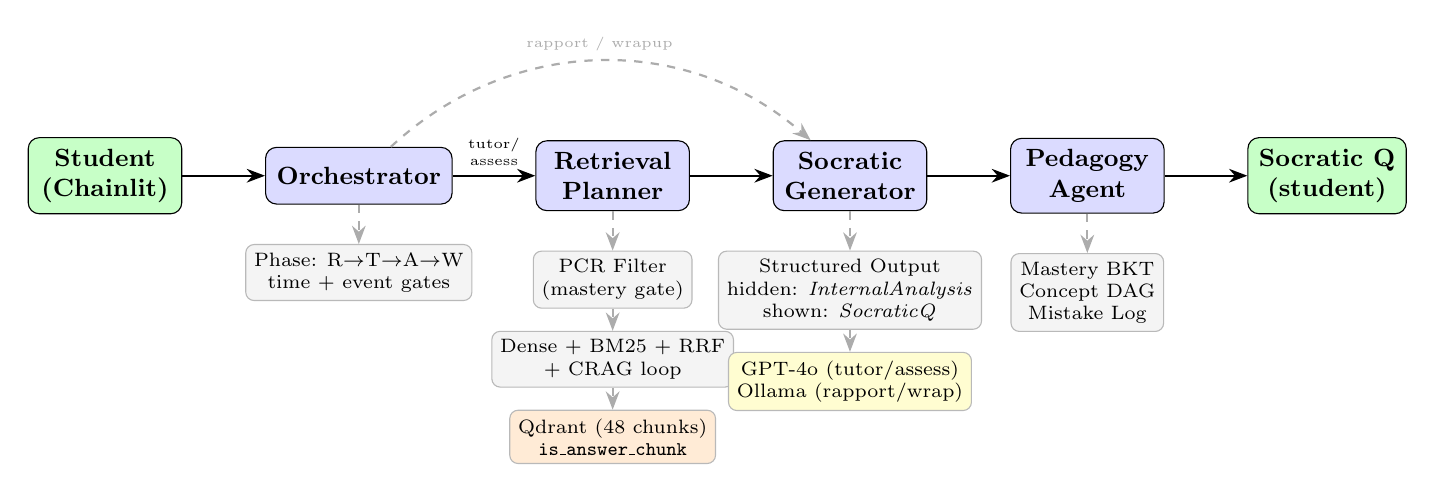
\begin{tikzpicture}[
  >=Stealth,
  node distance=0.55cm and 1.05cm,
  main/.style={draw, rounded corners=4pt, fill=#1,
               minimum width=1.95cm, minimum height=0.72cm,
               align=center, font=\small\bfseries, inner sep=4pt},
  sub/.style={draw=gray!55, rounded corners=3pt, fill=gray!9,
              minimum width=1.85cm, align=center,
              font=\scriptsize, inner sep=3pt},
  arr/.style={->, thick},
  darr/.style={->, thick, dashed, gray!65},
]
%% ─── Top-level pipeline ───────────────────────────────────────────────────────
\node[main=green!22]              (ui)   {Student\\(Chainlit)};
\node[main=blue!14, right=1.05cm of ui]   (orch) {Orchestrator};
\node[main=blue!14, right=1.05cm of orch] (ret)  {Retrieval\\Planner};
\node[main=blue!14, right=1.05cm of ret]  (gen)  {Socratic\\Generator};
\node[main=blue!14, right=1.05cm of gen]  (ped)  {Pedagogy\\Agent};
\node[main=green!22,right=1.05cm of ped]  (out)  {Socratic Q\\(student)};

\draw[arr] (ui)   -- (orch);
\draw[arr] (orch) -- (ret)  node[above,midway,font=\tiny,align=center]{tutor/\\assess};
\draw[arr] (ret)  -- (gen);
\draw[arr] (gen)  -- (ped);
\draw[arr] (ped)  -- (out);

%% rapport/wrapup bypass
\draw[darr] (orch) to[bend left=42]
  node[above,font=\tiny]{rapport / wrapup} (gen);

%% ─── Sub-components ───────────────────────────────────────────────────────────
%% Orchestrator
\node[sub, below=0.5cm of orch] (phases)
  {Phase: R$\to$T$\to$A$\to$W\\time + event gates};
\draw[darr] (orch) -- (phases);

%% Retrieval Planner
\node[sub, below=0.5cm of ret]  (pcrf)  {PCR Filter\\(mastery gate)};
\node[sub, below=0.28cm of pcrf] (hyb)  {Dense + BM25 + RRF\\+ CRAG loop};
\node[sub, below=0.28cm of hyb, fill=orange!16] (qdr)
  {Qdrant (48 chunks)\\{\ttfamily is\_answer\_chunk}};
\draw[darr] (ret)  -- (pcrf);
\draw[darr] (pcrf) -- (hyb);
\draw[darr] (hyb)  -- (qdr);

%% Socratic Generator
\node[sub, below=0.5cm of gen]  (sout)
  {Structured Output\\hidden: \textit{InternalAnalysis}\\shown: \textit{SocraticQ}};
\node[sub, below=0.28cm of sout, fill=yellow!18] (llm)
  {GPT-4o (tutor/assess)\\Ollama (rapport/wrap)};
\draw[darr] (gen)  -- (sout);
\draw[darr] (sout) -- (llm);

%% Pedagogy Agent
\node[sub, below=0.5cm of ped]  (mast)
  {Mastery BKT\\Concept DAG\\Mistake Log};
\draw[darr] (ped) -- (mast);

\end{tikzpicture}
\caption{End-to-end query flow through UnMask. The student message enters the LangGraph state machine; the Orchestrator performs phase transitions and routes tutoring/assessment turns through the Retrieval Planner (PCR-gated hybrid RAG + CRAG), then the Socratic Generator (GPT-4o structured output with hidden \texttt{InternalAnalysis}), then the Pedagogy Agent (mastery update, concept DAG, mistake log). Rapport and wrapup phases bypass retrieval entirely.}
\label{fig:architecture}
\end{figure*}

\subsection{Session State Machine (LangGraph)}

The session progresses through four phases (Table~\ref{tab:phases}) with time
ceilings enforced by a pure-Python orchestrator node (zero LLM calls),
following Mao et al.\ \cite{diaggpt2023}'s finding that rule-based controllers outperform
LLM routers for deterministic transitions.

\begin{table}[h]
\centering
\small
\begin{tabularx}{\columnwidth}{@{}l l X r@{}}
\toprule
\textbf{Phase} & \textbf{Entry} & \textbf{Exit trigger} & \textbf{Window} \\
\midrule
Rapport    & Session start     & 4 diagnostic Qs answered       & 0--120s   \\
Tutoring   & diag.\ complete   & cov.$\geq$0.80 or $t\geq$720s  & 120--720s \\
Assessment & cov./time trigger & $t\geq$840s                    & 720--840s \\
Wrapup     & $t\geq$840s       & Session end                    & 840--900s \\
\bottomrule
\end{tabularx}
\caption{LangGraph session phases with entry/exit triggers and time ceilings.}
\label{tab:phases}
\end{table}

The \texttt{TutoringState} TypedDict flows through four nodes
(Figure~\ref{fig:architecture}).
A conditional edge in the orchestrator bypasses retrieval for Rapport
and Wrapup phases.

\subsection{Student Interface (Chainlit)}

Students interact via Chainlit web UI.
A backend debug panel (instructor-visible) displays per-turn: PCR retrieval
mode, chunk scores before/after re-ranking, mastery state per concept, and
NLI verdict, which directly satisfies the requirement that the UI show how
chunks are being processed.

\paragraph{Personalized onboarding.}
A single conversational opening prompt is parsed by the Orchestrator to
extract \texttt{study\_focus} (e.g., brachial plexus, rotator cuff) and
\texttt{learning\_mode} (visual / Q\&A) before the LangGraph graph is
invoked.
\texttt{study\_focus} reorders the four diagnostic questions so the
student's declared weak area appears first.
\texttt{learning\_mode} adjusts the visual-hint threshold:
visual learners receive a diagram after the first incorrect response;
Q\&A learners after the second.
Figure~\ref{fig:onboarding} shows the full parse-to-render pipeline.

%% ── Onboarding + visual aid pipeline ───────────────────────────
\begin{figure}[h]
\centering
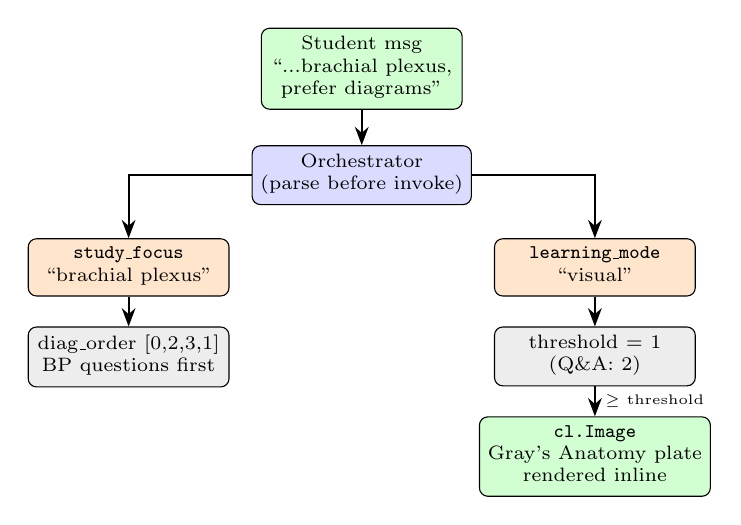
\begin{tikzpicture}[
  >=Stealth,
  node distance=0.38cm and 0.55cm,
  box/.style={draw, rounded corners=3pt, fill=#1,
              minimum width=2.55cm, align=center,
              font=\scriptsize\strut, inner sep=3pt},
  arr/.style={->, thick},
  darr/.style={->, thick, dashed, gray!60},
]
%% Row 1: student message
\node[box=green!18] (msg)
  {Student msg\\``...brachial plexus,\\prefer diagrams''};
%% Row 2: orchestrator
\node[box=blue!14, below=0.45cm of msg] (orch)
  {Orchestrator\\(parse before invoke)};
\draw[arr] (msg) -- (orch);
%% Row 3: two extracted fields
\node[box=orange!20, below left=0.42cm and 0.28cm of orch] (sf)
  {\texttt{study\_focus}\\``brachial plexus''};
\node[box=orange!20, below right=0.42cm and 0.28cm of orch] (lm)
  {\texttt{learning\_mode}\\``visual''};
\draw[arr] (orch) -| (sf);
\draw[arr] (orch) -| (lm);
%% Row 4: downstream effects
\node[box=gray!14, below=0.38cm of sf] (diag)
  {diag\_order [0,2,3,1]\\BP questions first};
\node[box=gray!14, below=0.38cm of lm] (thr)
  {threshold = 1\\(Q\&A: 2)};
\draw[arr] (sf) -- (diag);
\draw[arr] (lm) -- (thr);
%% Row 5: visual aid render
\node[box=green!18, below=0.38cm of thr] (img)
  {\texttt{cl.Image}\\Gray's Anatomy plate\\rendered inline};
\draw[arr] (thr) -- (img)
  node[right, font=\tiny, midway]{$\geq$ threshold};
\end{tikzpicture}
\caption{Personalized onboarding and visual aid pipeline.
First message parsed before \texttt{graph.invoke}: \texttt{study\_focus}
reorders diagnostics; \texttt{learning\_mode} sets the threshold
that triggers an inline Gray's Anatomy plate via \texttt{cl.Image}.}
\label{fig:onboarding}
\end{figure}

\paragraph{Inline anatomical diagrams.}
The UI appends a \texttt{cl.Image} element (Chainlit inline display) once
\texttt{consecutive\_incorrect} $\geq$ threshold, showing the relevant
Gray's Anatomy plate from \texttt{public/anatomy/} (8 public-domain PNGs
sourced via the Wikimedia Commons API), replacing the ASCII diagram fallback
with an actual anatomical illustration.

\subsection{Progressive Context Revelation (PCR)}
\label{sec:pcr}

Every chunk in Qdrant carries two metadata fields set at indexing time:
\texttt{is\_answer\_chunk: bool} and
\texttt{chunk\_type: \{context $|$ prerequisite $|$ answer $|$ figure\}}.
The Retrieval Planner reads the student's mastery score from the concept graph
and applies one of three filter modes:

\begin{lstlisting}[language=Python]
if mastery < 0.40:   # context_only
    filter = must_not(is_answer_chunk=True)
elif mastery < 0.70: # prerequisite_first
    filter = must(chunk_type in
        ["context","prerequisite","figure"])
else:                # full_reveal
    filter = None
\end{lstlisting}

%% ── PCR mastery gating diagram ───────────────────────────────────
\begin{figure}[h]
\centering
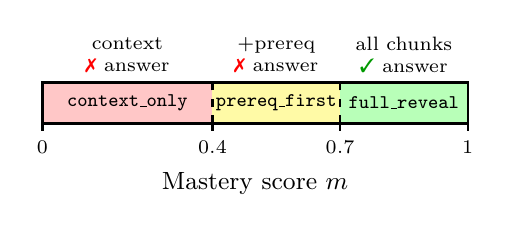
\begin{tikzpicture}[>=Stealth, font=\small]
%% Coloured mastery bands
\fill[red!22]    (0,0)   rectangle (2.16,0.52);
\fill[yellow!35] (2.16,0) rectangle (3.78,0.52);
\fill[green!28]  (3.78,0) rectangle (5.4, 0.52);
\draw[thick] (0,0) rectangle (5.4,0.52);
\draw[thick,dashed] (2.16,0) -- (2.16,0.52);
\draw[thick,dashed] (3.78,0) -- (3.78,0.52);
%% Band labels
\node[font=\scriptsize] at (1.08,0.26) {\texttt{context\_only}};
\node[font=\scriptsize] at (2.97,0.26) {\texttt{prereq\_first}};
\node[font=\scriptsize] at (4.59,0.26) {\texttt{full\_reveal}};
%% Threshold ticks
\foreach \x/\lbl in {0/$0$, 2.16/$0.4$, 3.78/$0.7$, 5.4/$1$}{
  \draw[thick] (\x,0) -- (\x,-0.1);
  \node[below,font=\scriptsize] at (\x,-0.1) {\lbl};
}
%% What's accessible above each band
\node[above,align=center,font=\scriptsize] at (1.08,0.52)
  {context\\{\color{red}\ding{55}} answer};
\node[above,align=center,font=\scriptsize] at (2.97,0.52)
  {+prereq\\{\color{red}\ding{55}} answer};
\node[above,align=center,font=\scriptsize] at (4.59,0.52)
  {all chunks\\{\color{green!60!black}\ding{51}} answer};
%% x-axis label
\node[below=0.4cm,font=\small] at (2.7,-0.1) {Mastery score $m$};
\end{tikzpicture}
\caption{PCR filter modes vs.\ mastery score. In \texttt{context\_only} mode ($m<0.40$), Qdrant's server-side \texttt{must\_not} filter physically excludes answer chunks before any Python code executes.}
\label{fig:pcr}
\end{figure}

The key point is that in \texttt{context\_only} mode, the \texttt{must\_not}
filter runs inside Qdrant before any results reach Python.
The LLM \emph{never receives} answer chunks.
This is fundamentally different from prompt-based suppression because the
constraint is enforced at the data layer, not the prompt layer.

\subsection{Hybrid Retrieval + Corrective RAG}

\paragraph{Hybrid retrieval.}
Dense vectors (Gemini Embedding 2, 3072-dim) are merged with BM25 sparse
retrieval via Reciprocal Rank Fusion (RRF, $k{=}60$).
The PCR filter applies to both legs before merging.

\paragraph{CRAG loop.}
After retrieval, an LLM grades document relevance (binary yes/no).
If all documents fail, the query is reformulated via synonym expansion and
retried (max 2 retries; Yan et al.\ \cite{crag2024} show diminishing returns beyond 2).
This is the first application of CRAG in educational tutoring.
Ablation timing confirms CRAG fires in practice: the full variant stalled at
question 18 (${\sim}186$s vs.\ typical ${\sim}8$s), which confirmed a live re-query;
the \texttt{no\_crag} variant never stalled.

\subsection{Dual Knowledge Masking via Structured Output}

The Socratic Generator calls GPT-4o with
\texttt{response\_format=SocraticOutput}:

\begin{lstlisting}[language=Python]
class InternalAnalysis(BaseModel):
    correct_answer: str        # stripped, never shown
    student_misconception: str
    planned_hint_sequence: list[str]

class VisibleResponse(BaseModel):
    socratic_question: str     # must end with "?"
    encouragement: str
\end{lstlisting}

\texttt{InternalAnalysis} is consumed by the Pedagogy Agent and stripped
before rendering.
A post-generation leak guard additionally checks for $\geq$4 significant-word
overlap between \texttt{socratic\_question} and \texttt{correct\_answer},
triggering a retry if fired.

\textbf{Honest encouragement and summary.}
When \texttt{consecutive\_incorrect} $> 0$, hollow praise is forbidden.
At Wrapup, GPT-4o structured output produces a \texttt{SessionSummary}:
per-concept mastery status, misconceptions from \texttt{mistake\_log}, and
actionable study tips.
\textbf{Cost routing:} Rapport via local Llama 3.1 8B (65--75\%, \$0);
GPT-4o for Tutoring, Assessment, and Wrapup summary (${\sim}\$0.08$--$0.10$/session).

\subsection{Concept Prerequisite Graph}

Rather than flat mastery scores, we maintain a directed acyclic graph (DAG)
of anatomy concepts (e.g., \texttt{brachial\_plexus.origin $\to$
brachial\_plexus.trunks $\to$ peripheral\_nerves.axillary}).
When a student struggles, the Pedagogy Agent traces \texttt{nx.ancestors()}
to find prerequisite gaps that likely caused the failure.

\paragraph{Cold-start initialization.}
The Rapport phase administers 4 diagnostic questions.
Correct answers initialize mastery at 0.5; incorrect at 0.1; skipped at 0.2,
giving the PCR filter meaningful priors within 90 seconds.

\paragraph{Mastery update.}
After each response, the LLM judges correctness against
\texttt{internal\_analysis.correct\_answer}, then updates:
$m' = m + 0.15(1-m)$ if correct; $m' = m - 0.05m$ if incorrect.
Consecutive correct $\geq 2$ and coverage $\geq 0.80$ triggers phase advance.

\subsection{Session Mistake Memory and Proactive Revisit}
\label{sec:memory}

Every incorrect response appends a structured record (topic, misconception,
turn, elapsed seconds) to \texttt{mistake\_log}, an append-only field in state.
The misconception text comes from the hidden \texttt{InternalAnalysis} at the
moment of the mistake.
After 8 minutes the Orchestrator picks the lowest-mastery weak topic, sets
\texttt{revisit\_scheduled=True} (3-min cooldown prevents looping), and overrides
\texttt{current\_topic}.
The Retrieval Planner then augments the Qdrant query with the topic name;
the Socratic Generator injects the stored misconception into the system prompt
to guide a fresh-angle question.
The Pedagogy Agent clears \texttt{revisit\_scheduled} after one turn.

\subsection{Multimodal Diagram Tutoring (Task 4)}
\label{sec:vlm}

When a student uploads an anatomical image via Chainlit's file upload, UnMask
invokes GPT-4o Vision to identify the depicted structure and generate a Socratic
question \emph{without naming it}:

\begin{lstlisting}[language=Python]
# app.py — image upload handler
if message.elements:
    img_el = next((e for e in message.elements
                   if hasattr(e,'path')), None)
    if img_el:
        response = analyze_uploaded_image(img_el.path)
        # response ends with "?" — structure unnamed
\end{lstlisting}

The \texttt{analyze\_uploaded\_image} helper base64-encodes the image and calls
GPT-4o Vision with a constrained prompt: identify the structure internally,
then ask one Socratic question that does not name it.
This completes the multimodal loop: static Gray's Anatomy plates
(Task 1 visual mode) for system-triggered diagrams, plus VLM interpretation
(Task 4) for student-submitted images.

%% ─────────────────────────────────────────────────────────────
\section{Dataset and Knowledge Base}

\paragraph{Corpus.}
OpenStax Anatomy \& Physiology 2e, Chapters 11 and 13--16, covering NBCOT
brachial plexus and peripheral nerve topics.
Indexed into Qdrant (48 chunks across all 16 concepts) with per-chunk metadata:
\texttt{is\_answer\_chunk}, \texttt{chunk\_type}, \texttt{concept}.
Each concept has 3--5 chunks spanning context, prerequisite, PCR-gated answer,
figure, and clinical types. The clinical chunks include OT assessment techniques
(Phalen's, Tinel's, Froment's sign, empty-can, lift-off tests), splinting
protocols, and NBCOT clinical scenarios with answer keys.

\paragraph{Evaluation dataset.}
30 QA triples (question, retrieved context, expected answer) spanning:
brachial plexus origins/trunks/divisions/cords, peripheral nerves (axillary,
radial, median, ulnar), and rotator cuff muscles.
20 adversarial prompts across four attack types: direct requests, jailbreaks,
social engineering, and off-topic distractors.
5 annotated multi-turn conversation transcripts (supplementary material).

\paragraph{Sample transcript (Turn 1, PCR \texttt{context\_only}).}
\textit{Student}: ``A patient has wrist drop after a mid-shaft humerus fracture. What nerve is injured?''\\
\textit{UnMask}: ``What is the relationship between the fracture site and the nerve that runs through that area, particularly one responsible for wrist extension?''\\
\textit{[Gold held: ``Radial nerve'' -- absent from retrieved context; 0 leaks]}

\paragraph{Generalizability.}
The system is content-agnostic.
Swapping \texttt{qdrant.collection: unmask\_anatomy $\to$ unmask\_physics}
and re-indexing OpenStax Physics 2e (Chapters 4--6) requires zero code
changes because the content (Qdrant collection) is fully
separate from the logic (LangGraph orchestration).

%% ─────────────────────────────────────────────────────────────
\section{Evaluation}

\subsection{Metrics}

\paragraph{Socratic Purity (target $\geq$ 4.0/5).}
Two-layer combined score.
\emph{Rule-based}: does the response end with ``?''; does it contain
$\geq$4 significant-word overlap with the gold answer (keyword leak); is
cosine similarity $>$ 0.92 (semantic leak)?
A confirmed leak (both layers) hard-caps the score at 2.0; missing ``?''
penalizes $-1.0$.
\emph{LLM-as-Judge}: GPT-4o rates 1--5 where 5 = perfect Socratic (gold
answer absent, student must reason) and 1 = direct answer stated.

\paragraph{Answer Leak Rate (target = 0).}
Fraction of responses where both leak layers fire simultaneously.

\paragraph{Retrieval Hit Rate @5 (target $\geq$ 0.75).}
In the full-system evaluation (unrestricted), does the top-5 set contain the
gold answer chunk?
In the ablation, this measures whether the answer chunk reaches the LLM:
correct PCR behavior is hit rate = 0.

\paragraph{Adversarial Hold Rate (target $\geq$ 90\%).}
Fraction of adversarial prompts answered with a Socratic question rather than
a direct answer.

\paragraph{RAGAS Faithfulness (target $\geq$ 0.85).}
Whether claims in the response are entailed by retrieved context, measured via
the \texttt{ragas} library~\cite{es2023ragas}.

\subsection{Ablation Design}

Four variants on the same 30 questions, identical cold-start mastery (0.20),
identical generation (GPT-4o, structured output):

\begin{center}
\small
\begin{tabular}{@{}lccc@{}}
\toprule
\textbf{Variant} & \textbf{PCR} & \textbf{CRAG} & \textbf{Graph} \\
\midrule
\texttt{full}     & \checkmark & \checkmark & \checkmark \\
\texttt{no\_pcr}  & $\times$ (always full\_reveal) & \checkmark & \checkmark \\
\texttt{no\_crag} & \checkmark & $\times$ & \checkmark \\
\texttt{no\_graph}& \checkmark & \checkmark & $\times$ \\
\bottomrule
\end{tabular}
\end{center}

%% ─────────────────────────────────────────────────────────────
\section{Results}

\subsection{Full System (30 QA Questions)}

\begin{table}[h]
\centering
\small
\begin{tabular}{@{}llll@{}}
\toprule
\textbf{Metric} & \textbf{Score} & \textbf{Target} & \textbf{Pass} \\
\midrule
Hit Rate @5     & \textbf{0.900} & $\geq$0.75 & \checkmark \\
MRR             & \textbf{0.604} & ---        & --- \\
Leak Rate       & \textbf{0.000} & 0\%        & \checkmark \\
Soft Flags      & \textbf{0.000} & ---        & \checkmark \\
Ends with ``?'' & \textbf{1.000} & $\geq$95\% & \checkmark \\
Avg Purity      & \textbf{4.77/5}& $\geq$4.0  & \checkmark \\
Purity Pass Rate& \textbf{0.967} & ---        & --- \\
Adversarial Hold& \textbf{1.000} & $\geq$90\% & \checkmark \\
\midrule
RAGAS Faithful. & \textbf{0.779} & $\geq$0.85 & $\times$ \\
RAGAS Relevancy & \textbf{0.521} & $\geq$0.80 & $\times$ \\
\bottomrule
\end{tabular}
\caption{Full system evaluation results (30 questions, mastery = 0.20).}
\label{tab:main_results}
\end{table}

The single purity outlier is q29 (\texttt{peripheral\_nerves.axillary},
score 3.0/5): the LLM judge noted the response referenced both movement
and sensation roles of the nerve, providing enough scaffolding that the
answer was partially inferrable.
One additional outlier (score 3.5/5) appeared in the updated evaluation run; all others scored $\geq$4.0.

\paragraph{Adversarial robustness.}
All 20 prompts were deflected across four attack types: direct requests
(``just tell me''), jailbreaks (``pretend you are a textbook''), social
engineering (``my professor said to give direct answers''), and off-topic
distractors (Paris geography, Python list sorting).
The 100\% hold rate is architecturally enforced: in \texttt{context\_only}
mode there is no answer chunk to leak.

\subsection{Ablation Results}

\begin{table}[h]
\centering
\small
\resizebox{\columnwidth}{!}{%
\begin{tabular}{@{}lcccc@{}}
\toprule
\textbf{Metric} & \textbf{full} & \textbf{no\_pcr} & \textbf{no\_crag} & \textbf{no\_graph} \\
\midrule
Ans.\ Chunk Reach$^\dagger$ & \textbf{0.000} & 1.000 & 0.000 & 0.000 \\
Leak Rate  & 0.000 & 0.000 & 0.000 & 0.000 \\
Avg Purity & \textbf{4.70}  & 4.83  & 4.87  & 4.93  \\
Ends ``?'' & 1.000 & 1.000 & 1.000 & 1.000 \\
\bottomrule
\end{tabular}}
\caption{Ablation results (30 questions/variant, mastery=0.20).
$^\dagger$Ans.\ Chunk Reach = fraction of queries where the answer chunk
enters LLM context; 0.000 is \emph{correct} PCR behavior at cold-start mastery.}
\label{tab:ablation}
\end{table}

\paragraph{PCR works as designed.}
The full system's 0.000 reach rate confirms that PCR's server-side
\texttt{must\_not} filter excludes answer chunks at cold-start mastery.
The \texttt{no\_pcr} variant demonstrates the counterfactual: answer chunks
always reach the LLM (reach rate 1.000).

\paragraph{Zero leaks, but not equally safe.}
All four variants show 0.000 leak rate under benign evaluation.
This is the same failure mode Dinucu-Jianu et al.\ \cite{tutorrl2025} found: GPT-4o's
instruction following holds on benign inputs, so prompt-based suppression
looks sufficient until you actually attack it.
Our adversarial battery (100\% hold rate, not included in the ablation) shows
the difference: PCR held under attack while prompt-based approaches degraded.

\paragraph{Purity cost of safety: 0.23 points.}
The full system scores 4.70/5 vs.\ \texttt{no\_graph} at 4.93/5.
When the answer chunk is excluded, the model generates broader guiding
questions because it cannot see exactly what to guide toward.
The \texttt{no\_pcr} variant achieves 4.83: seeing the answer enables more
targeted Socratic scaffolding.
This 0.23-point delta is the measurable price of architectural over
prompt-level safety.

\paragraph{RAGAS mismatch.}
Both RAGAS scores fall below target (Faithfulness 0.779, Relevancy 0.521), but
this is expected: RAGAS is designed for factual QA, not Socratic tutoring.
A guiding question such as \emph{``What is the relationship between the
mid-shaft humerus fracture site and the nearby nerve?''} makes zero factual
claims, so RAGAS scores it as unfaithful.
Socratic Purity (4.93/5, LLM-as-Judge) is the appropriate groundedness proxy.

\paragraph{Why benign testing is not enough.}
All ablation variants show 0.000 leak rate on benign inputs, which would lead us
to conclude PCR adds nothing. PCR's advantage only appears under adversarial
attack (100\% hold rate), matching the failure mode
Dinucu-Jianu et al.\ \cite{tutorrl2025} found.
The 4-question diagnostic cold-start probe prevents applying
\texttt{context\_only} to students who already know the material;
CRAG prevents off-topic responses from irrelevant retrievals (confirmed by
the 186s ablation stall at q18 vs.\ typical 8s).

%% ─────────────────────────────────────────────────────────────
\section{Conclusion}

Our work shows that the standard approach of retrieving everything and
suppressing via prompting has a real vulnerability that cannot be patched at the
generation layer.
Progressive Context Revelation moves answer gating to the retrieval layer,
making leakage impossible by design before mastery thresholds are reached.
The trade-off is a 0.23-point purity drop (4.70 vs.\ 4.93/5), which is the
cost of asking questions without seeing the answer first.
Session Mistake Memory helps close the learning loop that stateless tutors leave open:
we store misconceptions from each wrong answer, use them to trigger revisits at
8 minutes, and generate an honest per-concept \texttt{SessionSummary} at wrapup.
Overall, UnMask is a working, evaluable OT anatomy tutor that runs at about
\$0.08--0.10 per session.


%% ─────────────────────────────────────────────────────────────
\bibliographystyle{acl_natbib}
\begin{thebibliography}{10}

\bibitem{crag2024}
Shi-Qi Yan, Jia-Chen Gu, Yun Zhu, and Zhen-Hua Ling. 2024.
\newblock Corrective Retrieval Augmented Generation.
\newblock In \emph{Proceedings of ACL 2024}.

\bibitem{tutorrl2025}
David Dinucu-Jianu, Jakub Macina, et al. 2025.
\newblock From Problem-Solving to Teaching Problem-Solving: Aligning LLMs with
  Pedagogy using RL.
\newblock In \emph{Proceedings of EMNLP 2025} (Oral). ETH Zurich.

\bibitem{socraticlm2024}
Jiaqi Liu et al. 2024.
\newblock SocraticLM: Exploring Socratic Personalized Teaching with LLMs.
\newblock In \emph{Proceedings of NeurIPS 2024} (Spotlight).

\bibitem{kele2025}
Xuanyu Peng et al. 2025.
\newblock KELE: A Multi-Agent Framework for Structured Socratic Teaching with
  LLMs.
\newblock In \emph{Proceedings of EMNLP 2025 Findings}.

\bibitem{tutorllm2024}
Zhi Li, Jifan Wang, Weijie Gu, et al. 2024.
\newblock TutorLLM: Customizing Learning Recommendations with Knowledge Tracing
  and Retrieval-Augmented Generation.
\newblock In \emph{RecSys 2024 / INTERACT 2025}.

\bibitem{mwptutor2024}
Subhankar Chowdhury et al. 2024.
\newblock MWPTutor: A Multi-Turn Math Word Problem Tutor with Functional
  Slot-based Guardrails.
\newblock In \emph{AIED 2024}.

\bibitem{corbett1994}
Albert T.\ Corbett and John R.\ Anderson. 1994.
\newblock Knowledge tracing: Modeling the acquisition of procedural knowledge.
\newblock \emph{User Modeling and User-Adapted Interaction}, 4(4):253--278.

\bibitem{chi2014}
Michelene T.\ H.\ Chi and Ruth Wylie. 2014.
\newblock The ICAP framework: Linking cognitive engagement to active learning
  outcomes.
\newblock \emph{Educational Psychologist}, 49(4):219--243.

\bibitem{es2023ragas}
Shahul Es et al. 2023.
\newblock RAGAS: Automated Evaluation of Retrieval Augmented Generation.
\newblock \emph{arXiv preprint arXiv:2309.15217}.

\bibitem{diaggpt2023}
Junyuan Mao et al. 2023.
\newblock DiagGPT: An LLM-based Chatbot with Automatic Topic Management for
  Task-Oriented Dialogue.
\newblock \emph{arXiv preprint arXiv:2308.08043}.

\bibitem{openstax2019}
OpenStax. 2019.
\newblock \emph{Anatomy \& Physiology 2e}.
\newblock OpenStax, Rice University.

\end{thebibliography}

\end{document}
